\documentclass[../../main.tex]{subfiles} % Allows individual compilation
\graphicspath{{\subfix{../../images/}}}

\begin{document}

\section{Cas Homogène}
Avant de commencer, notons que comme $M$ est $\mathcal{O}(1)$ vis-à-vis $n$, 
alors $C_{ab} \rightarrow 1$ et par l'équation \ref{eq:variance} nous avons 
(déjà utilisant $q_i = q_0 \forall i$):
\begin{equation*}
	\var{\frac{V}{\sqrt n}} = \frac{\var{V}}{n} \rightarrow \frac{q_0^2 
	\left(1 - q_0^2 \right)}{n} 
\end{equation*}
C'est-à-dire, pour utiliser la formule donnée pour la densité du semi-cercle, 
nous devons normaliser $V / \sqrt n$ par $\sigma = q_0 \sqrt{1 - q_0^2}$.

\subsection{Condition d'existence de valeurs propres isolées} 
Pour déterminer une condition d'existence de valeurs propres isolées, 
nous procédons comme dans le cours. Nous faisons l'expansion de l'équation 
caractéristique
\begin{equation*}
	\det{\frac{B}{\sqrt n} - \lambda I_n} = 0.
\end{equation*}
Développons cette expression en utilisant l'équation \ref{eq:B}:
\begin{equation*}
\begin{gathered}
% Eq. 1
\det{
	\frac{q_0^2 J M J^t}{n} + \frac{V}{\sqrt n} - \lambda I_n
} = 0 \\
% Eq. 2
\therefore \quad \det{\frac{V}{\sqrt n} - \lambda I_n} \det{
	I_n + \frac{q_0^2 J M J^t}{n} \left( \frac{V}{\sqrt n} 
	- \lambda I_n \right)^{-1}
} = 0.
\end{gathered}
\end{equation*}
Maintenant, en utilisant l'identité de Sylvester,
\begin{equation*}
\det{\frac{V}{\sqrt n} - \lambda I_n} \det{
	I_n + \frac{q_0^2}{n} J^t \left( \frac{V}{\sqrt n} 
	- \lambda I_n \right)^{-1} J M
} = 0.
\end{equation*}
C'est l'heure d'utiliser l'hypothèse de la convergence vers la transformée de 
Stieltjes du semi-cercle, en faisant attention au fait de normaliser $V$:
\begin{align}
	J^t \left( \frac{V}{\sqrt n} - \lambda I_n \right) 
	&= J^t \left( \frac{\sigma V}{\sigma \sqrt n} - \sigma 
	\frac{\lambda}{\sigma} I_n \right) \nonumber \\
	&= \frac{1}{\sigma} J^t \left( \frac{V}{\sigma \sqrt n} 
	- \frac{\lambda}{\sigma} I_n \right)^{-1} J \nonumber \\
	&\rightarrow \frac{1}{\sigma} g_{sc} 
	\left( \frac{\lambda}{\sigma} \right) J^t J
	\label{eq:norm_iso}
\end{align}
D'où, en utilisant aussi le fait que le premier facteur n'aura pas de valeurs 
propres dehors le bulk (en normalisant $V$ on aura convergence p.s. vers la loi
du semi-cercle), on conclut (en utilisant $j_a^t j_a / n \to c_a$)
\begin{equation*}
	\prod_{i=1}^K \left(1 + \frac{q_0^2}{\sigma} M_{ii} c_i g_{sc} 
	\left( \frac{\lambda}{\sigma} \right) \right) = 0.
\end{equation*}
Cherchons une condition pour que l'un des termes de ce produit, disons le 
$i$-ème, devienne zéro:
\begin{equation}
	\left(1 + \frac{q_0^2}{\sigma} M_{ii} c_i g_{sc} \left( \frac{\lambda}
	{\sigma} \right) \right) = 0 \implies g_{sc}
	\left( \frac{\lambda}{\sigma} \right) 
	= - \frac{1}{\frac{q_0^2 M_{ii} c_i}{\sigma}}.
	\label{eq:zero}
\end{equation}
Or, pour $\lambda = 2 \sigma$ nous avons
\begin{equation*}
	g_{sc}(2) = - \frac{1}{2 \pi} \int_{-2}^2 \frac{\sqrt{4 - x^2}}{2 - x} 
	\, dx = - \frac{1}{2 \pi} \int_{-2}^2 \sqrt{\frac{2+x}{2-x}} \, dx = -1.
\end{equation*}
En plus, $g_sc$ est croissante et $\lim_{\lambda \to +\infty} g_{sc}(\lambda) 
= 0$. Ainsi, pour que l'équation \ref{eq:zero} ait une solution, il faut avoir
\begin{equation*}
	-1 \leq - \frac{\sigma}{q_0^2 M_{ii} c_i} \leq 0 \implies M_{ii} c_i 
	\geq \frac{\sigma}{q_0^2} = \frac{\sqrt{1 - q_0^2}}{q_0}.
\end{equation*}

\subsection{Valeurs asymptotiques des valeurs propres isolées}
Substituons l'expression trouvée à l'équation \ref{eq:zero} dans l'équation 
canonique associée à $g_{sc}$:
\begin{equation}
	- \frac{1}{\frac{q_0^2 M_{ii} c_i}{\sigma}} 
	= - \frac{1}{\frac{\lambda}{\sigma} 
	- \frac{1}{\frac{q_0^2 M_{ii} c_i}{\sigma}}} \implies \lambda 
	= q_0^2 M_{ii} c_i + \frac{1 - q_0^2}{M_{ii} c_i}.
	\label{eq:valasymp}
\end{equation}
Vérifions numériquement cette expression. Nous prenons un graphe de taille 
$n = 4000$ avec $k=3$ communautés, et $q_0 = 0.05$. Le spectre est illustré 
dans la Figure \ref{fig:vals_asymp}.

\begin{figure}
	\centering
	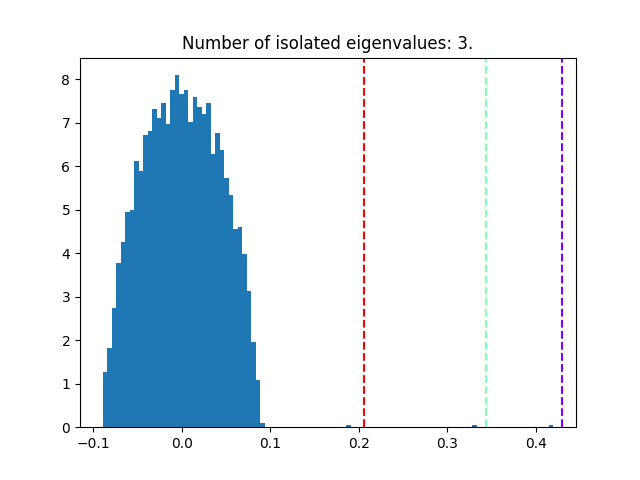
\includegraphics[width=0.65\textwidth]{../../images/cas_homogene/val_asymp/n_4000.png}
	\caption{Vérification numérique de l'expression des valeurs propres 
	asymptotiques}
	\label{fig:vals_asymp}
\end{figure}

\subsection{Alignements asymptotiques}
On determinera l'alignement asymptotique entre $\hat{u}_m$, un vecteur propre 
(empirique) isolé de $B / \sqrt n$, et le vecteur canonique $j_a$. Pour faire 
cela, nous évaluerons l'intégrale
\begin{equation*}
	\frac{1}{2 \pi i} \oint_{\Gamma_m} \frac{1}{n_a} j_a^t 
	\left( \frac{B}{\sqrt n} - z I_n \right)^{-1} j_a \, dz,
\end{equation*}
où le contour $\Gamma_m$ est un cercle autour la limite asymptotique $\rho_m$ 
pour la valeur propre isolée $\lambda_m$ de $B / \sqrt n$ et sans aucun autre 
valeur propre à son intérieur. Notons d'abord que
\begin{equation*}
	\left( \frac{B}{\sqrt n} - z I_n \right)^{-1} = \sum_i \frac{\hat{u}_i 
	\hat{u}_i^t}{\lambda_i - z}.
\end{equation*}
Alors, pour tous vecteurs $a$ et $b$,
\begin{equation*}
	a^t \hat{u}_m \hat{u}_m^t b = - \frac{1}{2 \pi i} \oint_{\Gamma_m} a^t 
	\left( \frac{B}{\sqrt n} - z I_n \right)^{-1} b \, dz.
\end{equation*}
En particulier pour les vecteurs canoniques,
\begin{equation*}
	\frac{1}{n_a} j_a^t \hat{u}_m \hat{u}_m^t j_a = -\frac{1}{2 \pi i} 
	\oint_{\Gamma_m} \frac{1}{n_a} j_a^t \left( \frac{B}{\sqrt n} - z I_n 
	\right)^{-1} j_a \, dz
\end{equation*}
Utilisons la formule d'inversion de Woodbury pour le terme inverse:
\begin{equation*}
\begin{gathered}
	\left( \frac{B}{\sqrt n} - \lambda I_n \right)^{-1} 
	= \left(\frac{q_0^2 J M J^t}{n} 
	+ \left( \frac{V}{\sqrt n} - z I_n \right) \right)^{-1} \\
	= Q(z) - Q(z) J \tilde M \left( I + J Q(z) J \tilde M \right)^{-1} 
	J Q(z),
\end{gathered}
\end{equation*}
où $Q(z) = \left(V / \sqrt n - z I_n \right)^{-1}$, et $\tilde M = q_0^2 / n M$.
Nous pouvons facilement manipuler cette expression à la forme
\begin{equation*}
	Q(z) - Q(z) J \left( \tilde M^{-1} + J^t Q(z) J \right)^{-1} J^t Q(z),
\end{equation*}
qui sera pratique car nous pourrons utiliser la convergence isotrope: si l'on 
fait attention à normaliser $V$ par $\sigma$, nous savons que $J^t Q(z) J \to 
\left( 1/\sigma \right) g_{sc}(z/\sigma) J^t J$ (voir l'équation 
\ref{eq:norm_iso}). En multipliant par $1 / n_a$, $j_a^t$ à gauche et par $j_a$
à droite, nous avons
\begin{equation*}
	\frac{j_a^t Q(z) j_a}{n_a} - \frac{1}{n_a} j_a^t Q(z) J 
	\left(\tilde M^{-1} + J^t Q(z) J \right)^{-1} J^t Q(z) j_a.
\end{equation*}
En intégrant cette expression, le premier terme devient zéro (car il est 
analytique à l'intérieur du contour), et l'autre devient (après une manipulation 
facile de multiplier et diviser par $n_a$ à l'intérieur du terme inverse):
\begin{equation}
	\frac{1}{2 \pi i} \oint_{\Gamma_m} \frac{1}{n_a^2} j_a^t Q(z) J 
	\left( \frac{n M^{-1}}{n_a q_0^2} + \frac{J^t Q(z) J}{n_a} \right)^{-1}
	J^t Q(z) j_a \, dz
	\label{eq:integrale}
\end{equation}
Or, analysons les pôles du terme intégré. Quand $n \to \infty$, il y aura une 
singularité quand quelque terme de la diagonale de l'inverse a une singularité 
à l'intérieur de $\Gamma_m$, c'est à dire, quand
\begin{equation*}
	\kappa_i (z) = \left( \frac{1}{c_a M_{ii} q_0^2} + \frac{1}{\sigma} g
	\left( \frac{z}{\sigma} \right) \frac{c_i}{c_a} \right)^{-1} 
	= \frac{1}{h_i (z)}
\end{equation*}
a une singularité à l'intérieur de $\Gamma_m$. Nous pouvons vérifier en 
substituant l'équation \ref{eq:zero} que cette singularité existera si, et 
seulement si, $i = m$ (en assumant que $M_{mm} \neq M_{ii}$ ou $c_i \neq c_m$).
Analysons son ordre et résidu.

Montrons que $\rho_m$ est un zéro de premier ordre pour $h_m(z)$. Or,  $h_m 
\left( \rho_m \right) = 0$ par la définition de $\rho_m$ à l'équation 
\ref{eq:zero}, et $h_m^\prime \left( \rho_m \right) \propto g_{sc}^\prime 
\left( \rho_m / \sigma \right) \neq 0$ car $g_{sc}^\prime (z) = g_{sc}^2(z)/
\left( 1 - g_{sc}^2(z) \right)$ et aussi par l'équation \ref{eq:zero} nous avons 
$g_{sc} \left( \rho_m / \sigma \right) \neq 0$. Alors $\rho_m$ est un zéro de 
premier ordre pour $h_m (z)$ et donc un pôle de premier ordre pour $\kappa_m (z)$. 
Son résidu est alors $\lim_{z \to \rho_m} \left( z - \rho_m \right) \kappa_m (z)$. 
Assumons encore que $h_m(z) = \left( z - \rho_m \right) f_m(z)$ pour quelque 
fonction $f_m(z)$ avec $f_m \left( \rho_m \right) \neq 0$. Alors
\begin{equation*}
	h_m^\prime (z) = f_m(z) + \left( z - \rho_m \right) f_m^\prime (z) 
	\implies f_m(z) = h_m^\prime(z) - \left( z - \rho_m \right) f_m(z),	
\end{equation*}
d'où, en substituant dans l'expression pour le résidu,
\begin{equation*}
	\lim_{z \to \rho_m} \left(z - \rho_m \right) \kappa_m (z) 
	= \frac{1}{h_m^\prime \left( \rho_m \right)} = c_a c_m 
	\left( q_0^2 M_{mm} \right)^2 - \sigma^2 \frac{c_a}{c_m} = R_m,
\end{equation*}
où nous avons défini $R_m$. La matrice inverse de l'équation \ref{eq:integrale} 
devient alors $e_m R_m e_m^t$, où $e_m$ est le m-ème vecteur canonique. Ainsi, 
l'intégrale de l'équation \ref{eq:integrale} devient, en utilisant le fait que 
$J e_m = j_m$:
\begin{equation*}
	\frac{1}{n_a^2} j_a^t Q(\rho_m) j_m R_m j_m^t Q(\rho_m) j_a \, dz \to 
	\frac{1}{n_a^2} \frac{1}{\sigma^2} g_{sc}^2 \left( \frac{\rho_m}{\sigma} 
	\right) \langle j_m, j_a \rangle^2.
\end{equation*}
En utilisant le fait que $\langle j_m, j_a \rangle^2 = n_a^2 \delta_{a=m}$ et 
en substituant l'expression pour $g_{sc}$, nous concluons
\begin{equation*}
	\frac{1}{n_a} j_a^t \hat u_m \hat u_m^t j_a = \delta_{a=m} \left( 1 - 
	\frac{\sigma^2}{\left( c_m q_0^2 M_{mm}^2 \right)^2} \right).
\end{equation*}

\subsection{Vérification numérique}
Vérifions numériquement ces alignements. Nous avons pris $n$ allant de $100$ 
jusqu'à $2000$ pour une matrice $M \sim 100$ fixée. Le résultat est affiché à 
la Figure \ref{fig:align_asymp}. Nous observons qu'une des convergences était 
lente. Cela se justifie quand on regarde les valeurs de $M$: $\diag{M} = 
\left( 237.8, 785.7, 655.0 \right)$. Alors la convergence lente probablement 
correspond à la communauté avec la valeur plus petite de $M$.

\begin{figure}
	\centering
	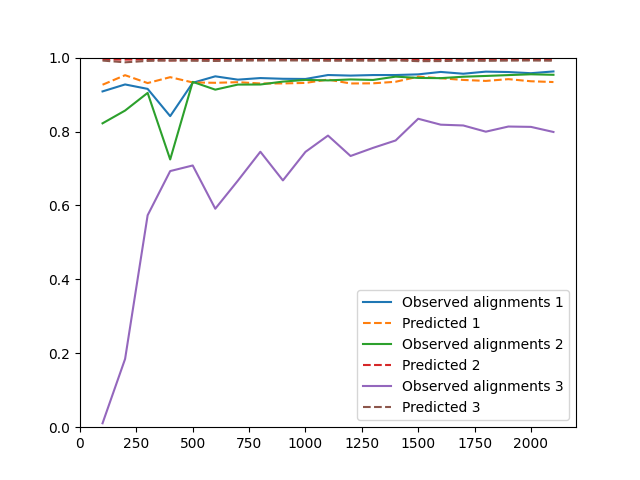
\includegraphics[width=0.65\textwidth]{../../images/cas_homogene/align_asymp/M_1000.png}
	\caption{Vérification numérique de l'alignment asymptotique entre les 
	trois vecteurs propres associés aux spikes et les vecteurs canoniques 
des classes}
	\label{fig:align_asymp}
\end{figure}

\subsection{Proposition d'un algorithme de détection de communautés}

Nous avons montré que les vecteurs propres liés aux valeurs propres isolées sont
alignés avec les vecteurs des classes. Ainsi, une idée d'algorithme de détection
de communautés consisterait à trouver les vecteurs propres isolés de la matrice
$B/\sqrt{n}$ et à utiliser un algorithme de clustering de $K$ classes, $K$-means
par exemple, pour clusteriser les $n$ lignes de la matrice des vecteurs propres
isolés. Ainsi, l'algorithme proposé de détection de communauté basé sur le
spectre consiste à
\begin{enumerate}
    \item Identifier les valeurs propres isolées du spectre de
	    $\frac{B}{\sqrt{n}}$. Extraire les vecteurs propres correspondants
	    $V = [v_1, ..., v_m] \in \mathbb{R}^{n \times m}$ avec $m < K$.
    \item Effectuer un $K$-means pour $K$ classes sur les vecteurs lignes de $V$.
\end{enumerate}
Un problème que nous pourrions rencontrer pour évaluer la performance de cet
algorithme est qu'il peut produire des classes avec des labels permutées par
rapport aux originales, donc une simple vérification de la précision ne serait
pas efficace. Nous proposons deux façons de résoudre ce problème : la première 
consiste à prendre la plus grande précision pour toutes les permutations 
possibles des labels. La seconde consiste à utiliser l'indice de Rand, une 
fonction qui mesure la similarité des deux affectations en ignorant les 
permutations. Dans la suite, nous avons décidé d'utiliser l'indice de Rand pour
mesurer les performances. Dans ce cas homogéne, on arrive a avoir en moyenne un
indice de Rand égal à $0.92$ pour $q_0 = 0.1$, $n= 3000$ et $M \sim 150$.

\end{document}
